\documentclass[12pt,a4paper]{article}

% 使用中文宏包
\usepackage[UTF8]{ctex}
\usepackage{graphicx} %插入图片的宏包
\usepackage{float} %设置图片浮动位置的宏包
\usepackage[strings]{underscore}
\usepackage{times}
\usepackage{epsfig}
\usepackage{amsmath}
\usepackage{amssymb}
\usepackage{overpic}
\usepackage{listings}
\usepackage{color}
\usepackage{enumitem}
\setenumerate[1]{itemsep=0pt,partopsep=0pt,parsep=\parskip,topsep=5pt}
\setitemize[1]{itemsep=0pt,partopsep=0pt,parsep=\parskip,topsep=5pt}
\setdescription{itemsep=0pt,partopsep=0pt,parsep=\parskip,topsep=5pt}

\definecolor{mygreen}{rgb}{0,0.6,0}
\definecolor{mygray}{rgb}{0.5,0.5,0.5}
\definecolor{mymauve}{rgb}{0.58,0,0.82}
\lstset{ %
  backgroundcolor=\color{white},   % choose the background color
  basicstyle=\footnotesize,        % size of fonts used for the code
  breaklines=true,                 % automatic line breaking only at whitespace
  captionpos=b,                    % sets the caption-position to bottom
  commentstyle=\color{mygreen},    % comment style
  escapeinside={\%*}{*)},          % if you want to add LaTeX within your code
  keywordstyle=\color{blue},       % keyword style
  stringstyle=\color{mymauve},     % string literal style
}

\usepackage[pagebackref=true,breaklinks=true,letterpaper=true,colorlinks,bookmarks=false]{hyperref}


\def\httilde{\mbox{\tt\raisebox{-.5ex}{\symbol{126}}}}


\graphicspath{{figures/}}

\setcounter{page}{1}

\begin{document}


%%%%%%%%% TITLE

\title{论文阅读笔记:隐私}
\author{纳文琪}
\maketitle


\section{Big Privacy: Challenges and Opportunities of Privacy Study in the Age of Big Data\cite{yu2016big}}

\subsection{引言}
\paragraph{} 最近研究表明,在大数据时代简单地匿名化数据集已无法再抵御针对隐私的攻击。保护隐私最直接的办法就是移除数据集中的ID,然而,事实表明这并不奏效。本质上,一个ID表示的是被描述对象的一组特征,但是实际上,我们依靠一个人的多种特征而不是ID来识别这个人。
\paragraph{隐私研究的两个方面} 隐私研究集中在两个方面:内容隐私(content privary)和行为隐私(interaction privacy)。
	\subparagraph{内容隐私} 攻击者根据受害者的一些知识背景从匿名或加密的数据集中识别受害者身份。
	\subparagraph{行为隐私} 攻击者更关注受害者的行为。
\paragraph{} 现代隐私研究主要关注两个方面:数据聚类(data clustering)和隐私框架(privacy framework)。


\subsection{基础知识}
\paragraph{隐私参与者} 包括:数据生产者、使用者、管理者、攻击者。
\paragraph{数据操作} 包括:收集、清洗(anonymizing)、交换(communicating)。
\paragraph{数据属性的类型} 包括:
	\subparagraph{显示标识(explicit identifier)} 比如身份证号、特定学校里的学号等;
	\subparagraph{准标识(quasi-identifier)} 通过关联其他数据集就可以确定用户的属性,比如性别、年龄等。我们一般将一个记录里面的所有准标识字段称为“qid”。拥有相同qid的值的一组记录被称为一个等价类(equivalent class)。
	\subparagraph{敏感信息(sensitive information)} 用户希望保护的那部分数据;
	\subparagraph{其他} 用户的其他信息。

\subsection{隐私研究的成果} 
\subsubsection{数据聚类方面}
\paragraph{} 数据聚类方面的研究成果主要包括:k-anonymity、l-diversity、t-closeness等。
\paragraph{k-anonymity} 首先,为保护隐私,我们必须将数据的ID全部移除,这样才能避免特定用户被识别。然而即便所有ID被移除,攻击者还是有可能通过诸如链接外部数据库等方式,根据qid来识别用户。k-anonymity方法的基本原则是:确保含有相同qid组数据的记录在数据集中至少出现k次,也就是说,每个等价类至少有k个记录。这样就可以使得攻击者通过qid识别特定用户的概率变为$\frac{1}{k}$,当存在一个很大的k值的时候,会对用户的识别产生一个很大的信息损失,从而达到隐私保护的作用。k-anonymity方法主要是用于处理准标识字段上的隐私保护问题,但不能处理敏感数据。攻击者可能使用同质攻击(homogeneity attach)或背景知识攻击(backgroud knowledge attack)来破解。
\paragraph{l-diversity} l-diversity方法可以克服k-anonymity方法的缺点。它要求数据集“对每一个qid的值,确保敏感数据字段至少有l个不同的值”。为了实现它,我们需要增大(还是减小?)敏感信息字段的颗粒度或增加噪声。某些特殊的时候,l-diversity会起到反作用,他会释放更多的信息增益给攻击者。
\paragraph{t-closeness} 可以修复l-diversity的脆弱性。它的基本思想是:对于任何一个等价类,保证它的值的分布被限定在t范围内。

\subsubsection{隐私框架方面}
\paragraph{微分隐私(differential privacy)} 在了解用户背景知识的情况下,攻击者可能会通过多次进行统计查询来获得期望的信息。防范策略是:对两个差别很小的数据集进行查询,其结果差别也应该很小,这样就可以限制攻击者获得的信息增益。
\paragraph{微分可识别性(differential identifiability)}
\paragraph{成员隐私(membership privacy)} 

\subsection{隐私研究的学科}

\subsection{隐私研究的数学描述}
\paragraph{匿名系统} 是一个映射函数:$F = X \rightarrow Y$,$X = \left \{ X_1,X_2,...,X_n \right \}$是原始数据,$Y=\left \{ Y_1,Y_2,...,Y_m \right \}$是系统的输出,对于攻击者,其目的是建立一个映射:$G: Y \rightarrow \hat X$,尽可能地从输出还原原始数据。
\paragraph{隐私保护系统的两个目的} 被描述为utility和privacy,这也是匿名系统F的两个关键指标。
	\subparagraph{utility} 使用 distorion D来度量,抽象地表示为:
	\begin{equation}
		D=\lambda(X;Y)
	\end{equation}
	D有很多种度量方法,例如,可以使用均方来表示。
	\subparagraph{privacy} 使用 leakage L 来度量,抽象地表示为:
	\begin{equation}
		L=\lambda(X;\hat X)
	\end{equation}
	L通常使用互信息来度量,即:
	\begin{equation}
		L=I(X,\hat X)
	\end{equation}
	
\paragraph{} 给定两个阈值$D_0$和$L_0$,匿名系统可作为一个优化问题:
\begin{equation}
  \begin{split}
  	optimize F \\
	s.t. \ D &\leq D_0 \\
	L &\leq L_0
  \end{split}
\end{equation}


\subsection{隐私度量(Privacy Measurements)}
\paragraph{}隐私的度量至今都没有太清晰的方法。现有以下几种度量方法:

	\subsubsection{相对度量(Relative Measurement)}
	\paragraph{} 其思想是:首先给定一个标准(benchmark),再度量研究对象到此标准的距离。比较流行的距离计算方式是Kullback-Leibler距离(相对熵)。
	\paragraph{} KL距离是基于一阶统计的度量方法,而二阶方法可以度量得更加精确。

	\subsubsection{信息论度量(Information Theoretic Measurement)}
	\paragraph{} 对于一个投票系统,定义三个随机变量V、S、E,分别表示投票者所投的票、来自投票系统以外的信息、攻击者由投票系统中获得的信息。
	\paragraph{完美隐私(perfectly privacy)} 定义为:在S条件下,V和E独立。即:$p_{V|S}(v;s) = p_{V|S,E}(v;s,e)$。
	\paragraph{隐私损失总量(amount of privacy loss)} 定义为:
	\begin{equation}
		L = \max (H(V|S) - H(V|S,E))
	\end{equation}
	度量隐私可能纰漏的程度。
	
	\subsubsection{Unicity Measure}

\subsection{隐私数学模型}

	\subsubsection{k-anonymity 模型}
	\paragraph{} 定义数据表$T=\left \{ t_1, t_2,...,t_n \right \}$ 是数据行的集合,$A=\left \{ A_1, A_2,...,A_n \right \}$ 是数据的属性集,$t_i[A_j]$表示元组$t_i$的属性$A_j$的值,$C=\left \{ C_1,C_2,...,C_k \right \} \subseteq A $是子属性集。定义 $T[C] = \left \{ t[C_1],t[C_2],...,t[C_k] \right \}$是t在C上的映射,$QI$为所有准标识符的集合。
	\paragraph{} 我们说一个表T满足k-anonymity,如果它满足,对于每一个元组$t \in T $ 都存在$k-1$个其他的元组$t_{i_1},t_{i_2},...,t_{i{k-1}} \in T $使得 $t[C]=t_{i_1}[C]=t_{i_2}[C]=...=t_{i_{k-1}}[C], C \subseteq QI$。也就是说,任何一组具有相同属性值的准标识符在表中至少出现k次。
	\subsubsection{l-diversity 模型}
	\subsubsection{t-closeness 模型}
	\subsubsection{Differential Privacy 框架}


\section{k-anonymity: A model for protecting privacy \cite{k-anonymity}}

\subsection{背景}
\paragraph{} 人们希望大量数据用于研究和分析,但同时又保证不泄露隐私,即同时满足“数据利用(utility)”和“保护隐私(privacy)”两个要求。通常,人们在发布数据时,会将数据集的标识符(如姓名、身份证号等)删去,从而使得数据集中的个体(individual)不能够被攻击者“重新识别(re-identify)”。然后,在很多情况下,利用非标识符字段仍然可以重新识别出个体。例如,研究显示,87\%的美国人可以通过邮编、性别和生日被识别出来。k-anonymity提供了一种避免此问题的框架。

\subsection{定义}
\paragraph{纰漏(disclosure)}指的是数据明显地或通过推理被意外地泄露。
\paragraph{纰漏控制(disclosure control)} 的目的是去识别或限制发布数据中的纰漏,也就是说,确保发布数据具有充分的匿名性。
\paragraph{准标识符(Quasi-identifier)} 如果数据表中的一组属性,可以通过与外部属性连接重新识别数据表中的个体,则称这组属性为准标识符。
\paragraph{准标识符的形式化定义} 令U为数据个体的全集,$T(A_1,...,A_n)$为数据表,存在两个映射$f_c: U \rightarrow T$和$f_g: T \rightarrow U'$,其中$U' \subseteq U$。表T的准标识符$Q_T$是一个属性集$\left \{ A_1,...,A_j\right \} \subseteq \left \{ A_1,...,A_n \right \}$,满足 $\exists p_i \in U $使得 $f_g(f_c(pi)[Q_T]) = p_i$。

\subsection{模型}
\paragraph{k-anonymity} 有表T和它的准标识符$Q_T$,当且仅当$T[Q_T]$中的每一行在$T[Q_T]$中至少出现k次时,我们说T满足k-anonymity。
\begin{figure}[H]
	\centering
	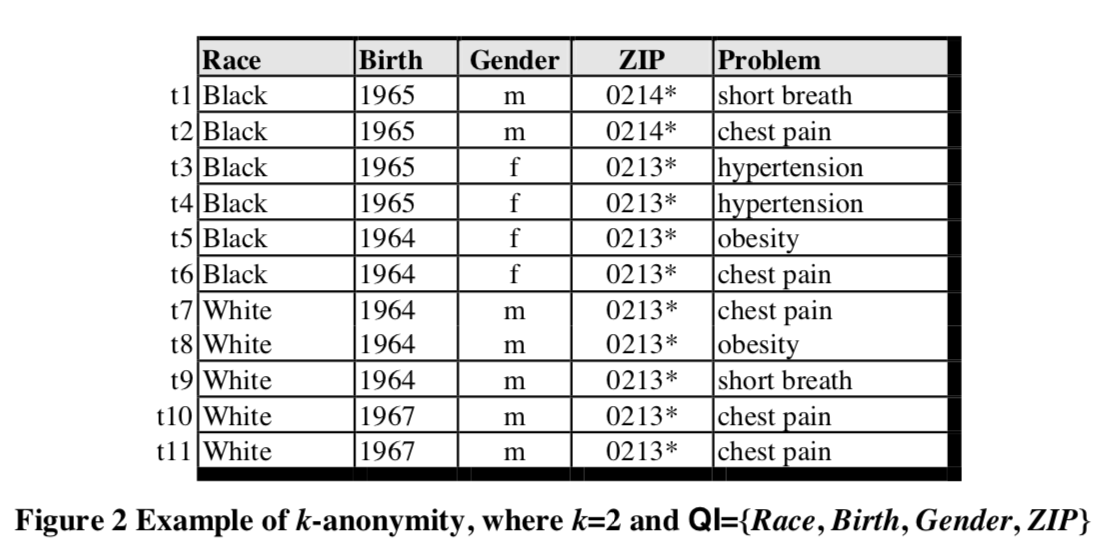
\includegraphics[width=0.7\textwidth]{../images/k-anonymity-example.png}
	\caption{}
	\label{}
\end{figure}

\subsection{攻击k-anonymity}
\paragraph{未排序匹配(Unsorted matching)攻击} 如果发布的表的数据的顺序固定,就可以根据这种固定顺序,关联多个发布的表来获取敏感信息。避免这种攻击很简单,只需要对数据进行乱序操作后再发布即可。
\paragraph{}





\bibliographystyle{ieeepes}
\bibliography{../Saliency}
\end{document}



























































